\section{Long Term Monitoring}

\begin{frame}{Our Proposal: PocketSniffer}
  \begin{figure}
    \centering
    \begin{tikzpicture}
      \node[anchor=south west,inner sep=0] at (0,0)
      {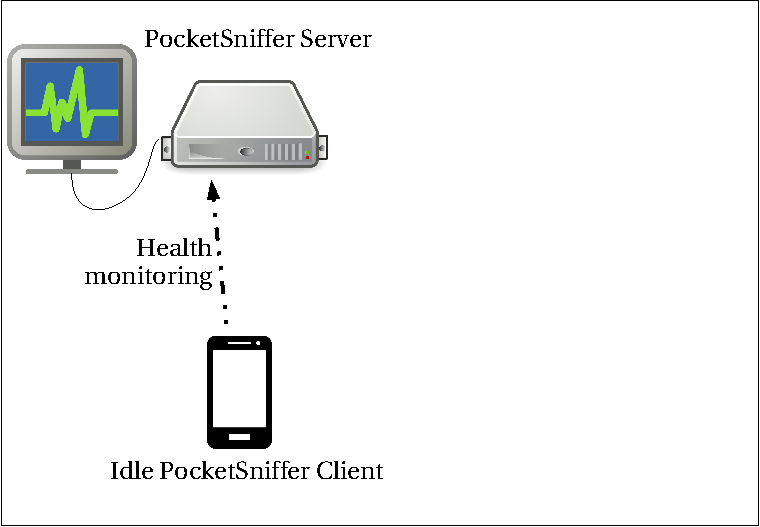
\includegraphics[width=0.6\textwidth]{system-1}};
    \end{tikzpicture}
  \end{figure}
  \textbf{Long-term large scale network monitoring.}
  \begin{itemize}
    \item Network health, performance, etc.
  \end{itemize}
  \color{gray}
  Short-term local spectrum management.
  \begin{itemize}
    \item \color{gray} Sniff the spectrum on behalf of nearby devices.
    \item Help with channel assignment, rate adaption, etc.
  \end{itemize}
\end{frame}


\begin{frame}{\Large Monitoring {\Huge Large} Wireless Network}
  \huge\textbf{\ldots is Hard.}\normalsize
  \begin{block}{If you want to know}
    \begin{itemize}
      \item Whether APs are alive? Easy\textendash SNMP\footnotemark.
      \item How APs are doing? Not so easy.
        \begin{itemize}
          \item \textbf{Client perceived} coverage and performance.
          \item Site surveys? Nay\ldots
        \end{itemize}
      \item Implication of "rogue" Access Points.
        \begin{itemize}
          \item Malicious? Easy, eliminate them all.
          \item Am I not doing good enough? Not so easy.
        \end{itemize}
    \end{itemize}
  \end{block}
  \huge Smartphones to the rescue!

  \large
  Always on, mostly idle, capture real user experience.
  \footnotetext[1]{Simple Network Management Protocol}
\end{frame}

\begin{frame}{Sounds Good. But\ldots}
  \Large
  \begin{itemize}
    \item \textbf{What} can smartphones measure?
      \begin{itemize}
        \item Monitoring capabilities.
      \end{itemize}
    \item \textbf{How} do we conduct and collect measurements?
      \begin{itemize}
        \item When and what to collect?
        \item Extra measurements needed?
      \end{itemize}
  \end{itemize}
  \begin{center}
    \Huge Does this even work?
  \end{center}
\end{frame}

\begin{frame}{Smartphone Capabilities}
  \begin{block}{What smartphones can measure}
    Network Health.
    \begin{itemize}
      \item Wifi scan results (AP visibility and signal quality).
      \item Link quality.
    \end{itemize}
    Network performance.
    \begin{itemize}
      \item Latency.
      \item Bandwidth.
    \end{itemize}
  \end{block}
\end{frame}

\begin{frame}{How to Collect?}
  Smartphones already perform \textbf{aggressive} network exploration.
  \begin{block}{Analysis of PhoneLab Wifi Dataset }
    \begin{itemize}
      \item 139 Android devices over 5 months (11/2013\textendash 4/2014).
      \item 88~M Wifi scan results, 300~K Wifi sessions.
    \end{itemize}
  \end{block}

  \begin{columns}[t]
    \begin{column}{0.48\textwidth}
      \vspace{0pt}
      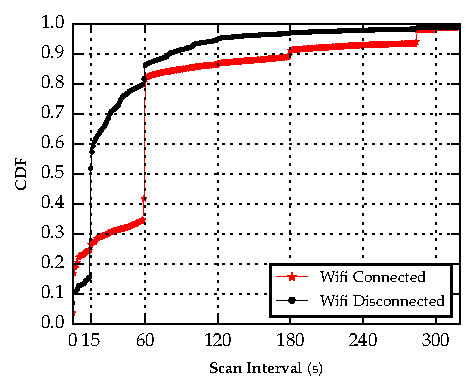
\includegraphics[width=\textwidth]{scan_interval}
    \end{column}%
    \begin{column}{0.52\textwidth}
      \vspace{0pt}
      \begin{itemize}
        \item 80\% of scan intervals $<$ 1 min.
        \item Take the free ride!
      \end{itemize}
      Performance measurement.
      \begin{itemize}
        \item Latency (RTT by cheap \texttt{ping}).
        \item Bandwidth.
      \end{itemize}
    \end{column}
  \end{columns}
\end{frame}

\begin{frame}{Case Studies}
  How does client-side measurement help monitoring networks?
  \begin{columns}
    \begin{column}{0.49\textwidth}
      \vspace{0pt}
      \begin{figure}
        \caption{AP Dominance}
        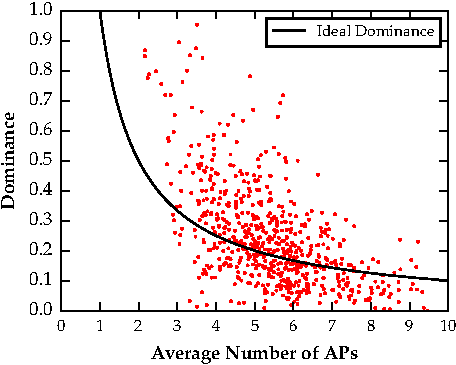
\includegraphics[width=\textwidth]{ap_dominance}
      \end{figure}
    \end{column}%
    \begin{column}{0.51\textwidth}
      \vspace{0pt}
      \begin{figure}
        \caption{Wifi Session Signal}
        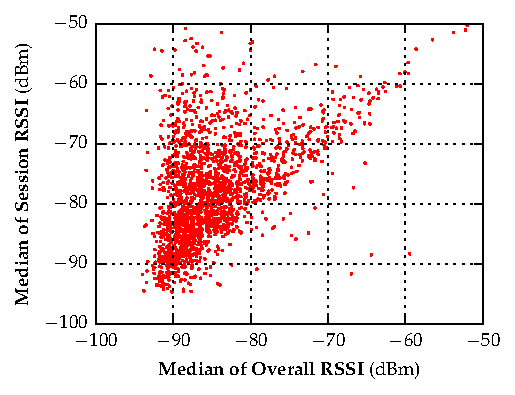
\includegraphics[width=\textwidth]{session_rssi}
      \end{figure}
    \end{column}

  \end{columns}
\end{frame}


\begin{frame}{Today}
  \LARGE
  \begin{itemize}
    \item Long-term network monitoring
    \item \textbf{Short-term spectrum management}
    \item Challenges and Progress
  \end{itemize}
\end{frame}
